%
% Lab Report - Template
%
% (c) 2004 EMT
% (c) 2013 SAT-IST-AAU
%
%---------------------------------------------------------
%
% This \LaTeX template can be used as a basis for the lab report.
%
%----------------------------------------------------------
%
\documentclass[12pt,a4paper,english]{article}

\usepackage{satlab}
\usepackage{siunitx}
\usepackage{amsmath}
\usepackage{ marvosym }
\usepackage{array} 
\usepackage{booktabs} 
\usepackage{hyperref}
%
\begin{document}

%---------------------------------------------------------
\MTHeader                           %  Please fill in!
%----------------------------
{Final Report}                    %  Exercise Title
%----------------------------
{Group B \\}                           %  Group-Nr.
%----------------------------
{Bozhidar Bozhikov \\ Nikita Smolianinov \\ Vladyslav Uhrik \\}
%----------------------------
{Dr. Narendiran Anandan\\ Serkan Ergun}         %  Supervisor
%----------------------------
{\today}                            %  Lab Date {\today}
%---------------------------------------------------------
%
\clearpage

\tableofcontents % if you want
\clearpage
%
\pagestyle{plain}
%

\begin{center}
{KS Basic Lab: Robot Design\hfill SS 2025}\\[1.5ex]
\end{center}
\section{Task Description (Bozhidar Bozhikov)}

The goal behind this project is to design a circular robot (diam. = ~30cm) with nominal speed 100mm/s. The robot must also fullfill the following requirements: 

\begin{itemize}
  \item[a)] be able to clear gaps of 6cm,
  \item[b)] be able to operate in darkness,
 \item[c)] be able to run for a minimum of 15 minutes,
 \item[d)] have line-tracking capability,
 \item[e)] have RC capability,
 \item[f)] be able to give acoustic feedback (~75dB)
 \item[g)] have maximum weight 800g,
 \item[h)] fit in a budget of 300\EUR
\end{itemize}

The design we decided to develop is inspired by real-world screw-propelled vehicles, which are moved with the help of a pair of rotating helix-shaped cylinders made of soft plastic or rubber. The cylinders have a spiral form like the thread of a screw which make contact with the ground. Motion is produced by the inverse of the screw conveyor: one cylinder's helix runs clockwise and the other - counterclockwise. Rotation is done with the activation of only one of the corresponding cylinders. This form of propulsion is used in real life to move through difficult terrain such as ice, mud, snow and water. As such, our robot would ideally operate on carpet (simulating mud and swamp) or on very smooth ground (simulating ice). 

The github repository used can be found \href{https://github.com/2-hardcore-4-u/RobotDesign2025}{here}. 

%\begin{figure}[!ht]
%  \begin{center}
%    \includegraphics[width=5.5cm]{./Figures/Kegel.png}
%    \caption{Figure 1 \label{fig:1}
%  \end{center}
%\end{figure}
%

\section{Specifications (Bozhidar Bozhikov, Vladyslav Uhrik)}

\subsection{Physical Calculations (Vladyslav Uhrik)}

\paragraph{Step 1: Define Requirements}
Target speed = 0.1 m/s (100 mm/s)
Helix pitch (measured or estimated) = 2 cm = 0.02 m
Robot mass = 0.8 kg
Wheel radius = 6 cm = 0.06 m
Surface type = linoleum or carpet friction coefficient $\mu$=0.4

\paragraph{Step 2: Calculate Required RPM}

We assume 1 full revolution of the helix moves the robot forward by 1 pitch length.

\begin{align*}
    \text{Revolutions per second (RPS)} &= \frac{\text{Linear speed}}{\text{Helix pitch}} = \frac{0.1}{0.02} = 5 \, \text{rev/sec}
\end{align*}

\textit{Helix pitch} = the axial distance (i.e., forward movement along the wheel's centerline) that the thread travels in one full \( 360^\circ \) rotation around the wheel.

\begin{align*}
	\text{RPM = 5 * 60 = 300 RPM}
\end{align*}

\paragraph{Step 3: Calculate Normal Force per Wheel}

Assume equal weight distribution across two wheels:

\begin{align*}
    F_N &= \frac{m \cdot g}{2} \\
        &= \frac{0.8\,\text{kg} \times 9.81\,\text{m/s}^2}{2} \\
        &= 3.924\,\text{N}
\end{align*}

\paragraph{Step 4: Calculate Friction Force (Required to Move)}

\begin{align*}
    F_{\text{friction}} &= \mu \cdot F_N \\
                        &= 0.4 \times 3.924\,\text{N} \\
                        &= 1.57\,\text{N}
\end{align*}

\paragraph{Step 5: Calculate Required Torque per Wheel}

\begin{align*}
    \tau &= F \cdot r \\
         &= 1.57\,\text{N} \times 0.06\,\text{m} \\
         &= 0.0942\,\text{Nm}
\end{align*}

Apply Safety Margin (1.5×)

\begin{align*}
    \tau_{\text{safe}} &= 0.0942 \times 1.5 \\
                       &= \SI{0.1413}{\newton\meter}
\end{align*}

\paragraph{Step 6: Convert RPM to Angular Velocity}

\begin{align*}
    \omega &= \frac{2\pi \times \text{RPM}}{60} \\
           &= \frac{2\pi \times 300}{60} \\
           &= \SI{31.42}{\radian\per\second}
\end{align*}

\paragraph{Step 7: Calculate Mechanical Power per Motor}

\begin{align*}
    P &= \tau \times \omega \\
      &= \SI{0.1413}{\newton\meter} \times \SI{31.42}{\radian\per\second} \\
      &= \SI{4.44}{\watt} \text{ per motor}
\end{align*}

\paragraph{Total Power for 2 Motors}

\begin{align*}
    P_{\text{motors}} &= 2 \times \SI{4.44}{\watt} \\
                      &= \SI{8.88}{\watt}
\end{align*}

\subsection{Electrical Power Calculations (Vladyslav Uhrik)}

\paragraph{Step 8: System Power Budget}

We calculate the power P of each component using the formula: $P = VI$

\begin{table}[h]
\centering
\caption{Component Power Consumption}
\label{tab:power_consumption}
\begin{tabular}{l S[table-format=1.3] S[table-format=1.3] S[table-format=2.3] p{4cm}}
\toprule
\textbf{Component} & \textbf{V (\si{\volt})} & \textbf{I (\si{\ampere})} & \textbf{P (\si{\watt})} & \textbf{Notes} \\
\midrule
ATmega32 & 5.0 & 0.020 & 0.10 & Powered from 5V rail \\
8P MCU & & & & \\
\addlinespace

nRF24L01 & 3.3 & 0.012 & 0.04 & Powered from 3.3V rail \\
P RF module & & & & \\
\addlinespace

VL53L1X & 2.8 & 0.019 & 0.05 & Direct 2.8V rail or onboard LDO \\
ToF sensor & & & & \\
\addlinespace

TP4056 & 5.0 & 1.000 & 5.00 & During charging (input) \\
charger module & & & & \\
\addlinespace

MT3608 & 12.0 & 0.010 & 0.12 & Estimated conversion overhead \\
(regulator loss) & & & & \\
\addlinespace

IIM-42652 & 3.3 & 0.007 & 0.023 & Motion tracking \\
\addlinespace

CNY70 & 5.0 & 0.018 & 0.09 & IR sensor (emitter + transistor) \\
IR sensor & & & & \\
\addlinespace

Buzzer (passive) & 5.0 & 0.030 & 0.15 & Approx. 75 dB \\
\addlinespace

2x Pololu Stepper & 2.8 & 3.400 & 9.52 & Two motors: $1.7\,\si{\ampere} \times 2$ \\
Motors & & & & \\
\bottomrule
\end{tabular}
\end{table}

Total Power = 24.613 W

\paragraph{Step 9: Energy Required for 15 Minutes}

Convert 15 min to hours:

\begin{align*}
E = 24.613 * 0.25 = 6.15325 Wh
\end{align*}

\paragraph{Step 10: Calculate Battery Capacity at 12V}

\begin{align*}
    C &= \frac{6.15325}{12} \\
      &= \SI{512.77}{\milli\ampere\hour}
\end{align*}

Add 30\% Safety Margin:

\begin{align*}
    C_{\text{safe}} &= 512.77 \times 1.3 \\
                    &= \SI{666.6}{\milli\ampere\hour}
\end{align*}

\begin{itemize}
    \item Voltage: \SI{12}{\volt}
    \item Minimum capacity: \SI{670}{\milli\ampere\hour} (rounded up) (we end up using a \SI{1000}{\milli\ampere\hour} battery)
\end{itemize}

\section{Hardware and CAD (Nikita Smolianinov)}

The Fusion model discussed in this section can be found in the .stp file. The robot's design follows real-world screw-propelled vehicles such as the  ZIL-2906 and other Amphirols. The circular mount of the robot is made from 4mm thick plywood, with the propulsion cylinders attached with a custom 3D-printed mount, which are driven by 2 bipolar stepper motors, chosen for their power and precision. The stepper motors provide 3 degrees of movement. 

\begin{figure}[!ht]
  \begin{center}
    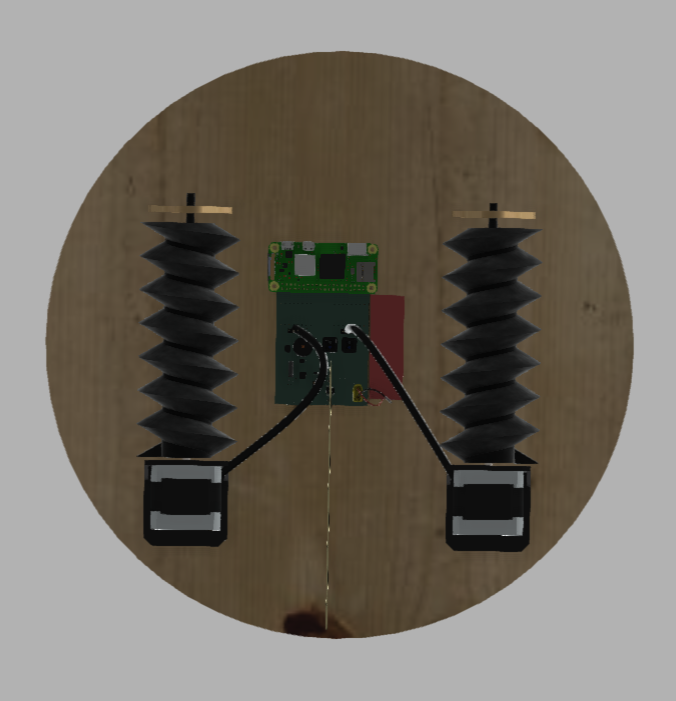
\includegraphics[width=5.5cm]{./Figures/cad.png}
    \caption{Bottom-down view of the CAD model.}
  \end{center}
\end{figure}

\section{PCB (Bozhidar Bozhikov)}

The circuits and PCB layout discussed in this section can be found in the PCB folder.

We chose a Raspberry Pi 4 Compute Module as our microcontroller for ease of integration and programming since it fit the budget, connected externally via a 40-pin array on our custom PCB. Connected to the microcontroller are a 6-axis IMU, time-of-flight sensor, two motor drivers for out screw-propulsion helical cylinders, an RF transciever for control, two infra-red reflective optical sensors to ensure line-tracking even in darkness as stated in the requirements and a buzzer. Additionally, since the motors operate at 12V, the microcontroller at 5V, and most of the components at 3.3V, we also included a 5V step-down converter and a 3.3V fixed-output regulator. The exact components and their respective datasheets can be found in the BillOfMaterials folder. 

The following circuits were designed by following the Application Examples in their respective datasheets and then connecting them to the microcontroller via GPIO pins. The raspberry's pinout is as follows:

\begin{itemize}
    \item GPIO08: RF chip select
    \item GPIO09: RF MISO
    \item GPIO10: RF MOSI
    \item GPIO11: RF clock
    \item GPIO12: IR sensor 1
    \item GPIO13: IR sensor 2
    \item GPIO22, GPIO23: pulse input (STEP) and direction control (DIR) respectively for motor 1
    \item GPIO24, GPIO25: pulse input (STEP) and direction control (DIR) respectively for motor 2
    \item GPIO26: buzzer
    \item GPIO27: RF enable

\end{itemize}

\begin{figure}[!ht]
  \begin{center}
    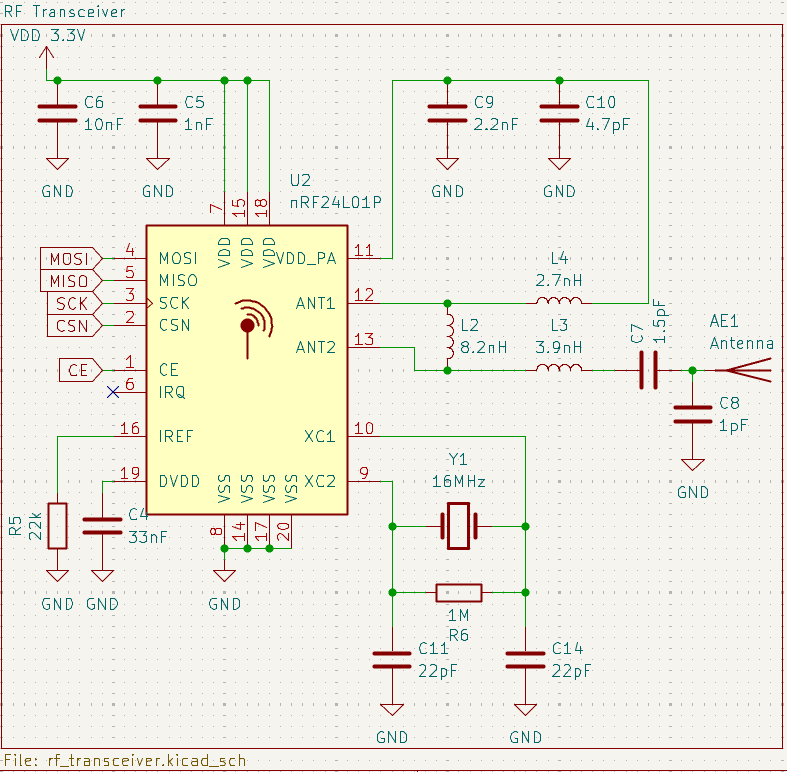
\includegraphics[width=5.5cm]{./Figures/rf.png}
    \caption{nRF24L01+ single-chip RF transciever, featuring a 16Mhz clock and an antenna.}
  \end{center}
\end{figure}

\begin{figure}[!ht]
  \begin{center}
    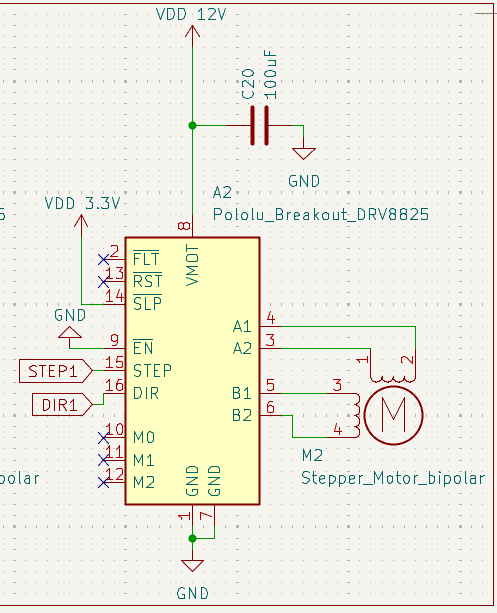
\includegraphics[width=5.5cm]{./Figures/motor.png}
    \caption{Motor driver sub-circuit.}
  \end{center}
\end{figure}

\begin{figure}[!ht]
  \begin{center}
    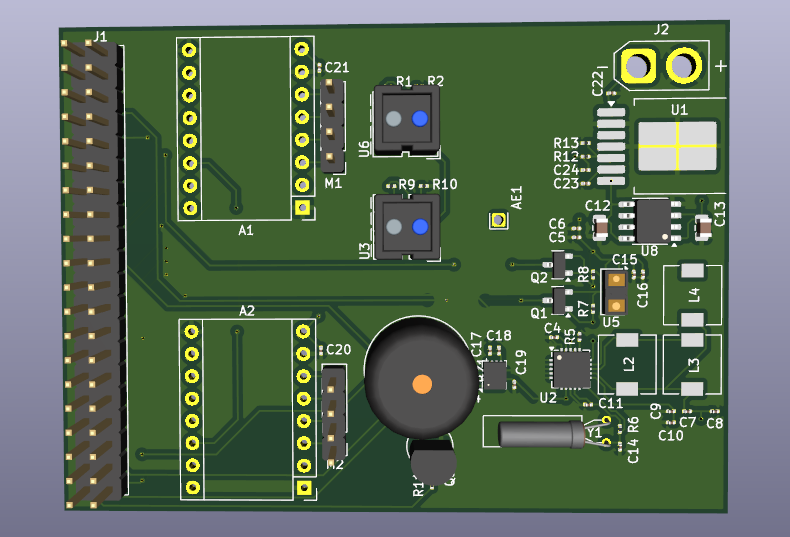
\includegraphics[width=5.5cm]{./Figures/pcb.png}
    \caption{Top-down view of the custom pcb.}
  \end{center}
\end{figure}

\section{Discussion (Bozhidar Bozhikov)}

The robot discussed in this report follows a real-world practical, albeit unorthodox, design utilizing the screw conveyor mechanism for propulsion on rough carpeted surfaces or smooth ground with 3 degrees of movement.


%
%-----------------------------------------------
% Bibliography
%

%\bibliographystyle{plaindin}
%\bibliography{bibFile}
\end{document}
